\section{Ablaufdiagramme}

\subsection{Import von Daten}

Dieses Sequenzdiagramm beschreibt den Verlauf des Imports von Daten vom "Upload"-Button aus.
Dazu wird erst der Import-Controller aufgerufen.
Dort wird mit den Informationen von der Weboberfläche eine Konfiguration erstellt und damit der UploadHandler aufgerufen.
Dieser konvertiert erst die Daten aus der Quelldatei in die interne Darstellung und arbeitet die zurückgegebene Table dann zeilenweise ab.
Die Daten werden mit dem Konfigurationsobjekt den richtigen Spalten zugeordnet und interpretiert.
Anschließend werden aus den Results und der ZonedDateTime Observations im ObservationCreator erstellt.
Diese werden mit der CheckDuplicate-Klasse auf Duplikate im FROST-Server überprüft und anschließend auf dem FROST-Server erstellt.

\begin{figure}[htbp]
\centering
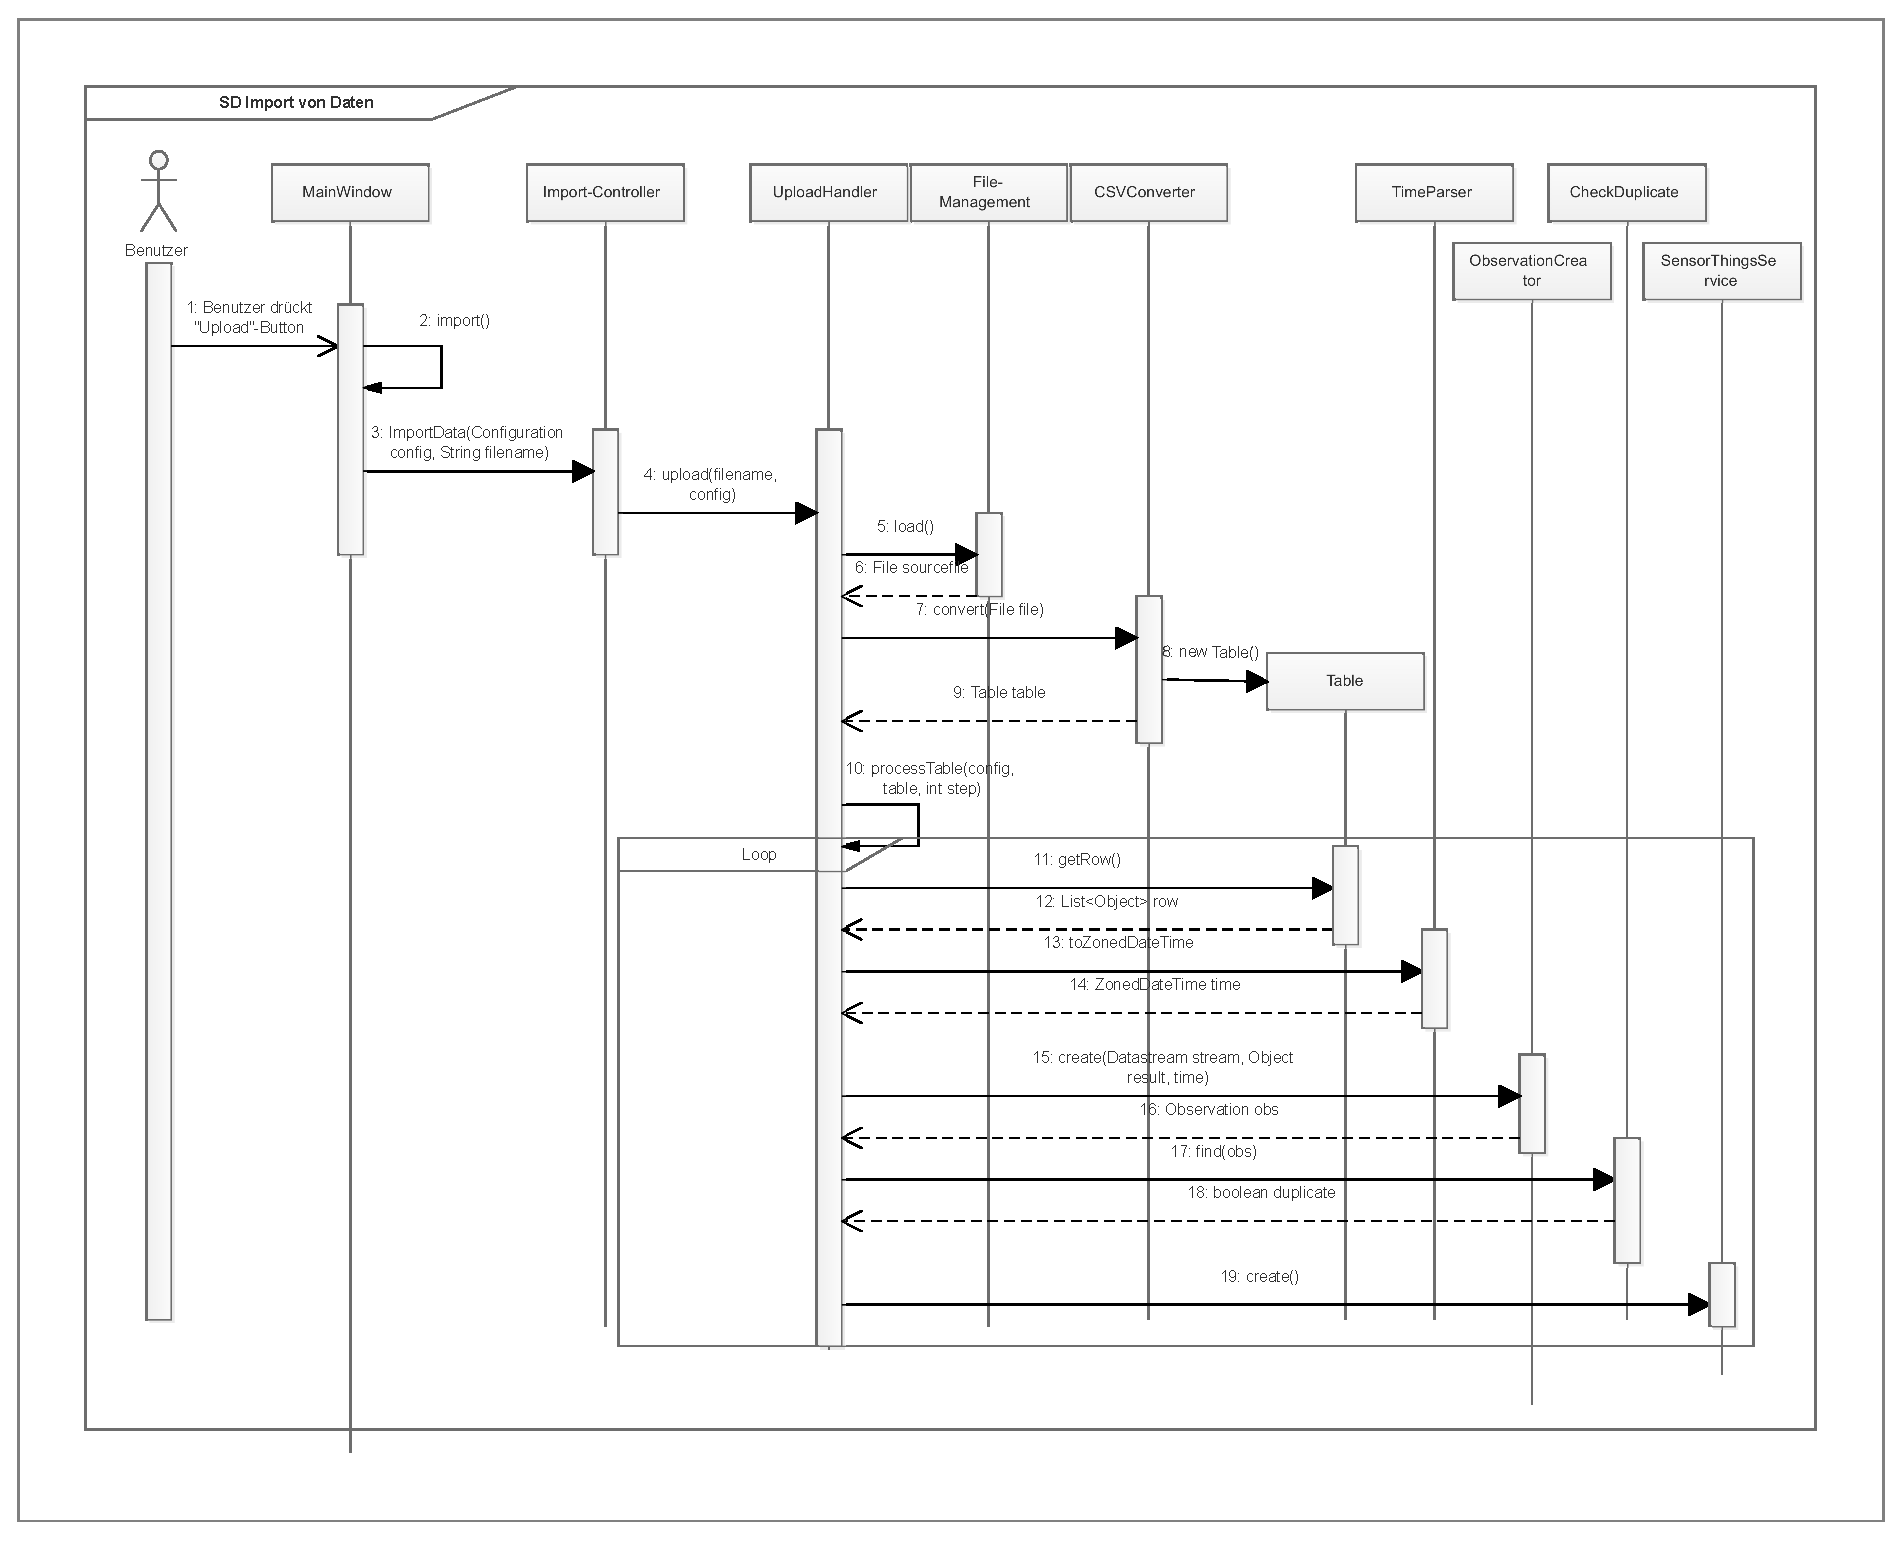
\includegraphics[scale=0.44]{uml/SD_upload.eps}
\caption{Sequenzdiagramm zum Upload von Daten auf dem FROST-Server}
\end{figure}

\clearpage
\subsection{Konfiguration speichern}
\begin{figure}[htbp]
\centering
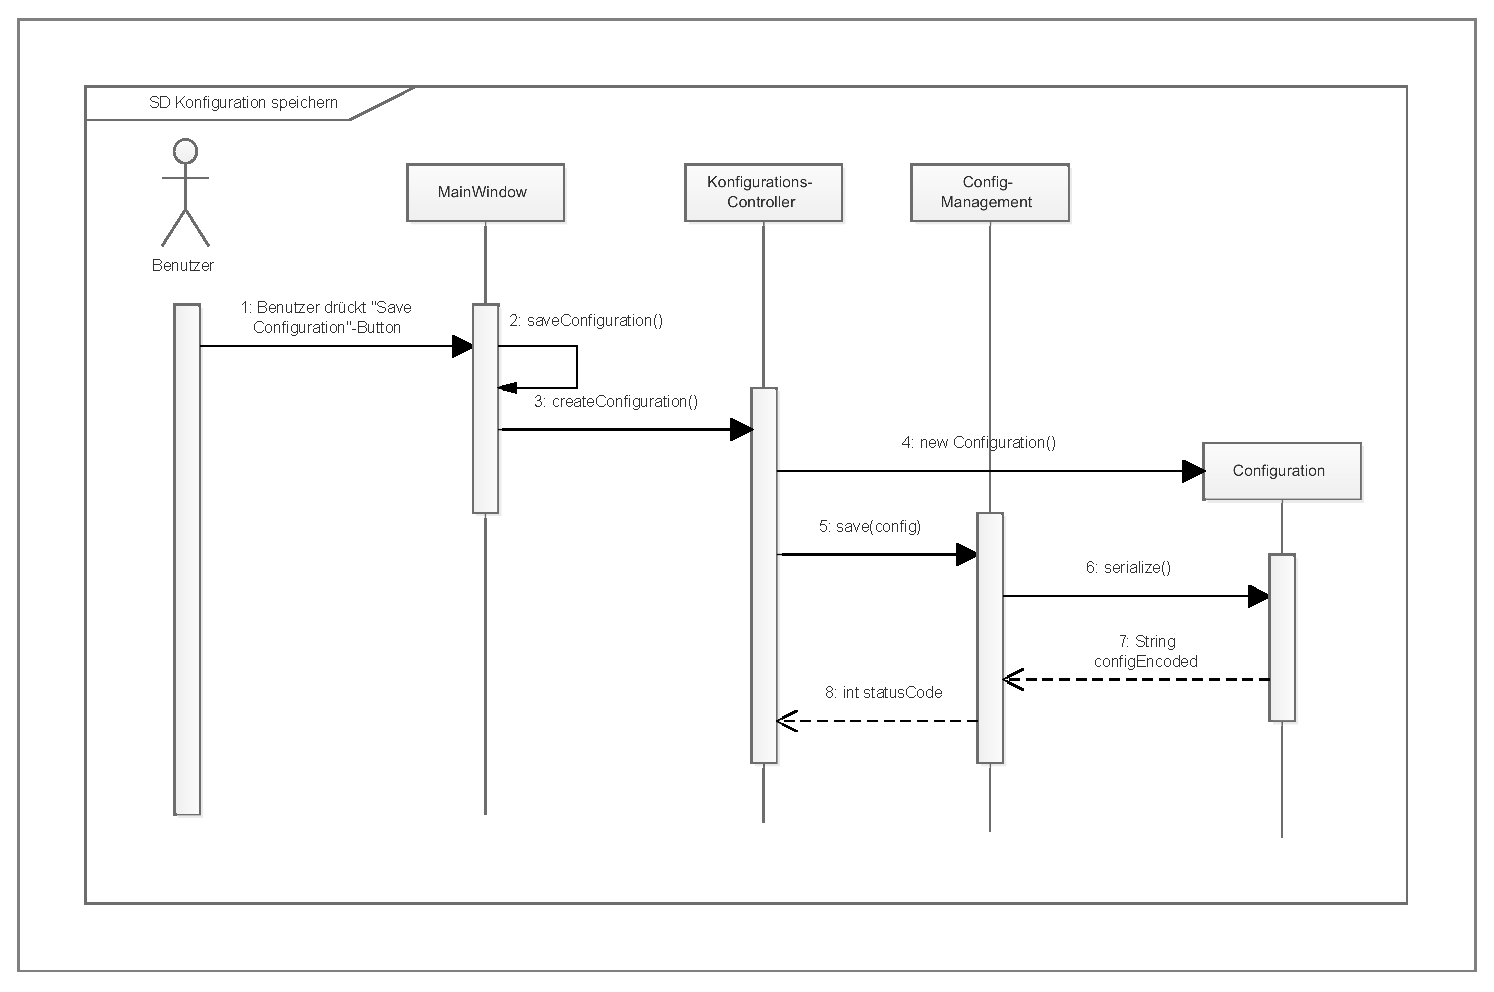
\includegraphics[scale=0.44]{uml/SD_saveConfig.eps}
\caption{Sequenzdiagramm zum Speichern einer Konfiguration}
\end{figure}

\clearpage
\subsection{Fehlerhafte Zeilen zurückgeben}
\begin{figure}[htbp]
\centering
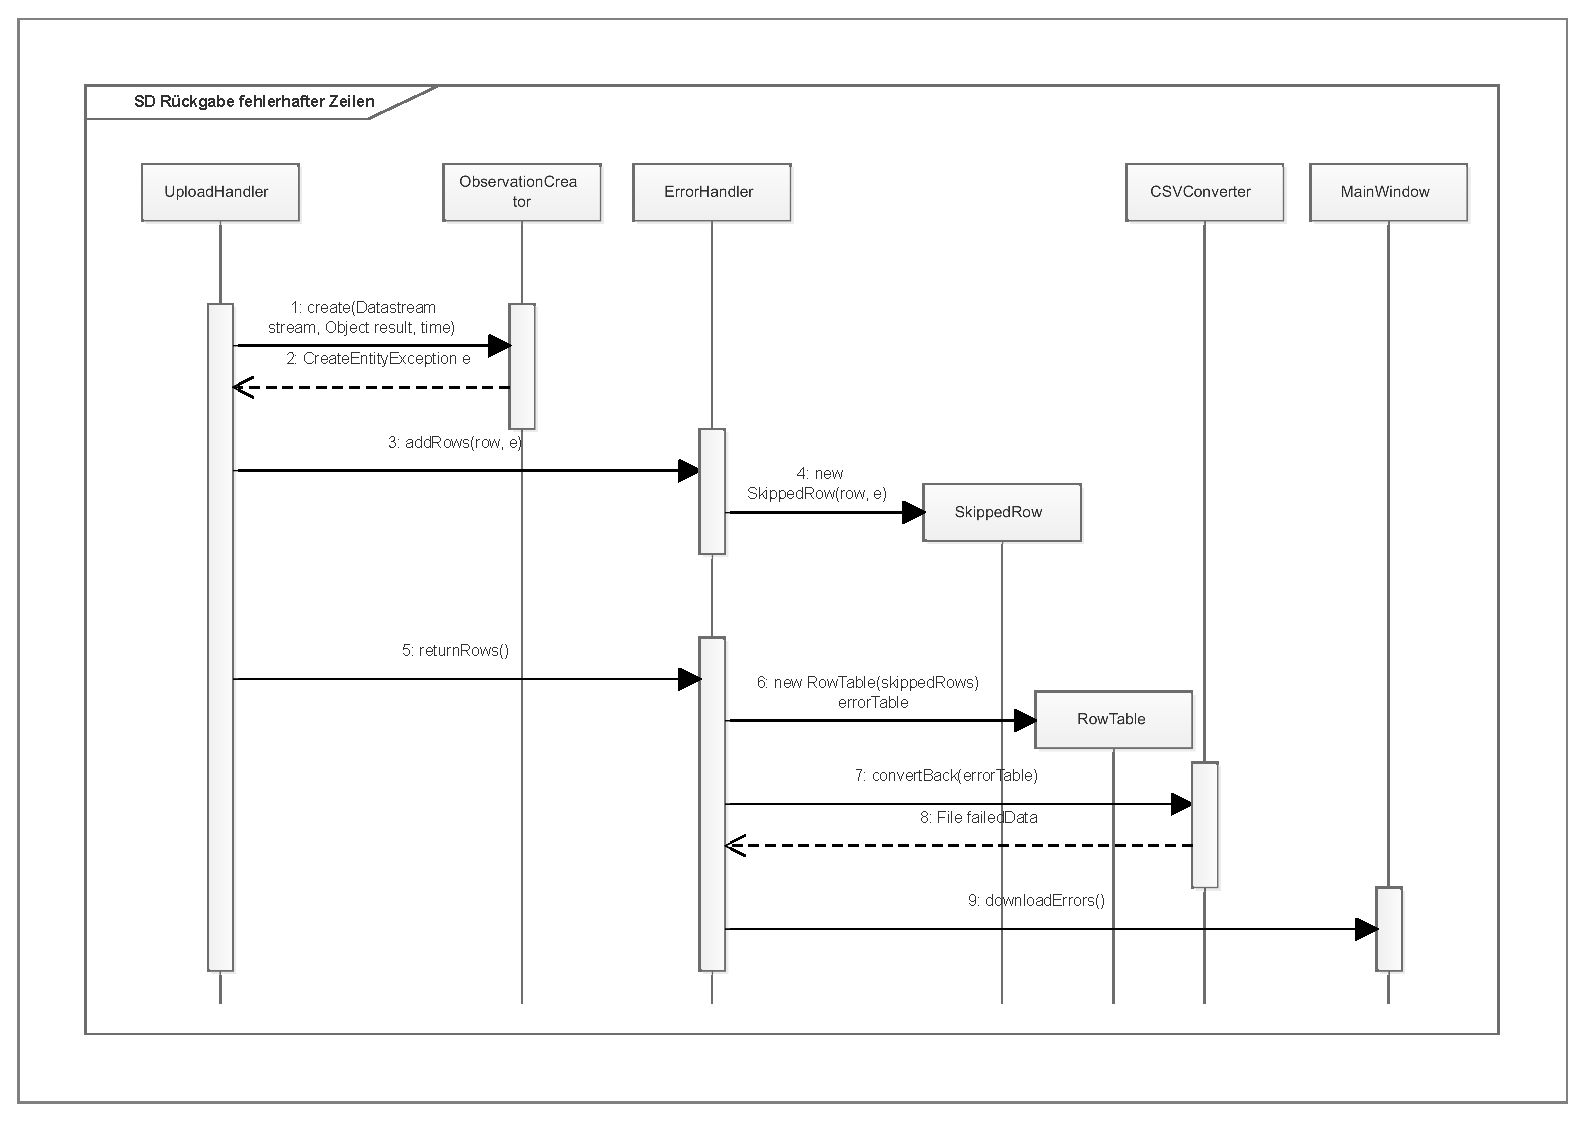
\includegraphics[scale=0.44]{uml/SD_returnErrors.eps}
\caption{Sequenzdiagramm zum Zurückgeben fehlerhafter Zeilen als Datei}
\end{figure}

\clearpage
\subsection{Thing erstellen}
\begin{figure}[htbp]
\centering
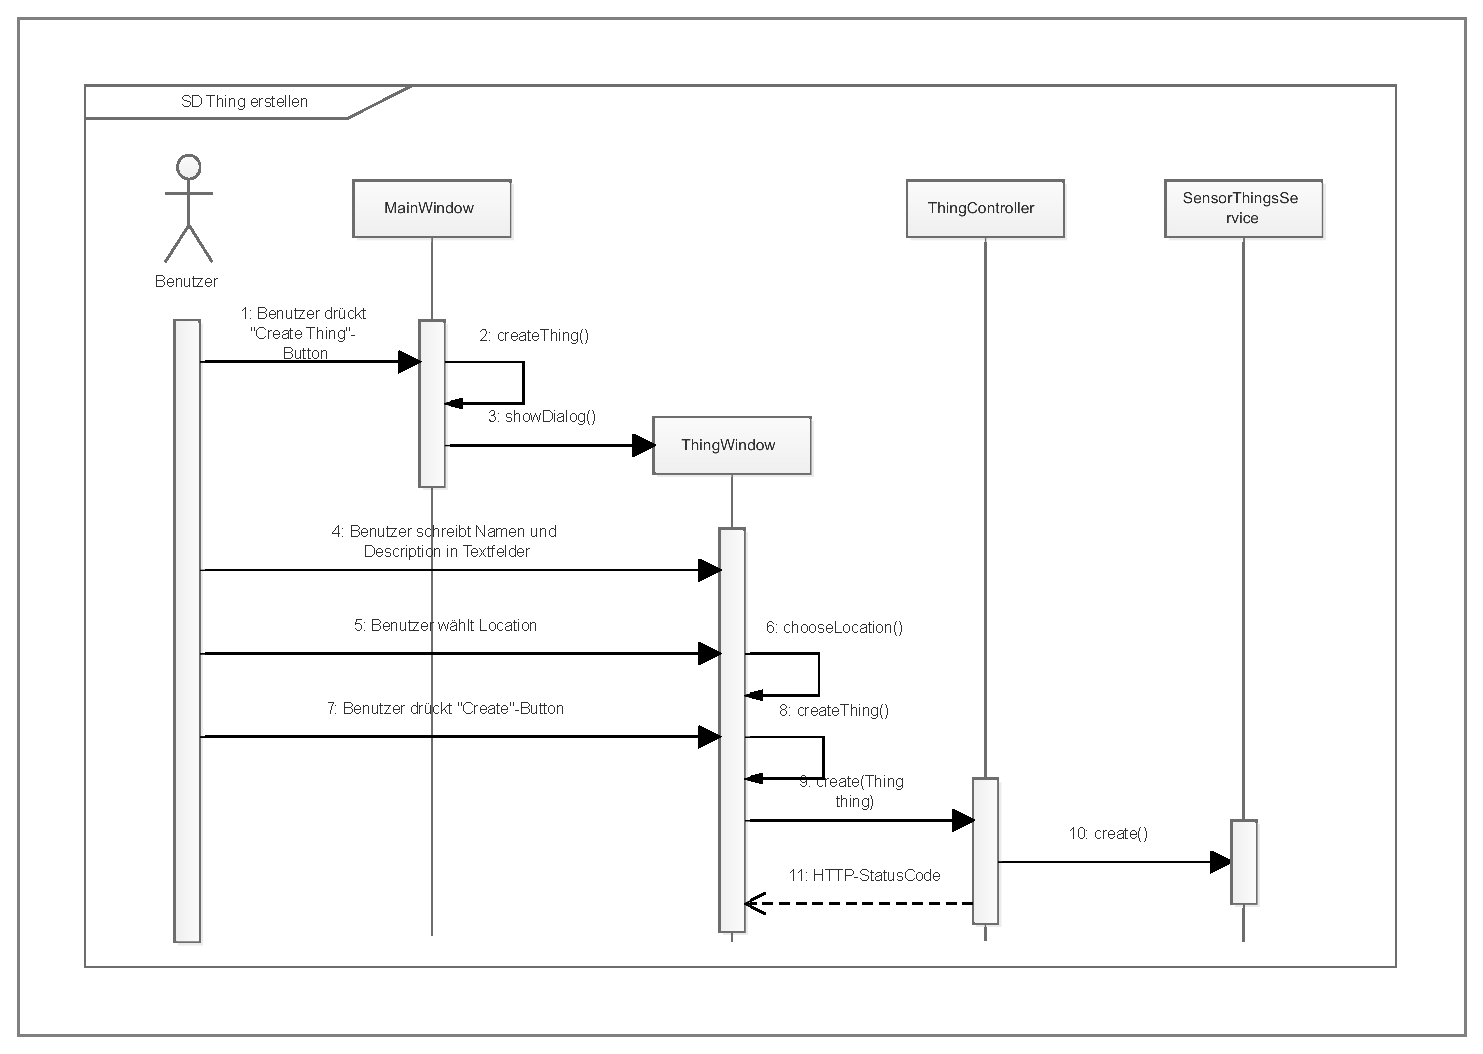
\includegraphics[scale=0.44]{uml/SD_createThing.eps}
\caption{Sequenzdiagramm zum Erstellen eines Things auf dem FROST-Server}
\end{figure}